\begin{figure}[H]
    \centering
    \begin{minipage}[t]{0.45\textwidth}
        \centering
        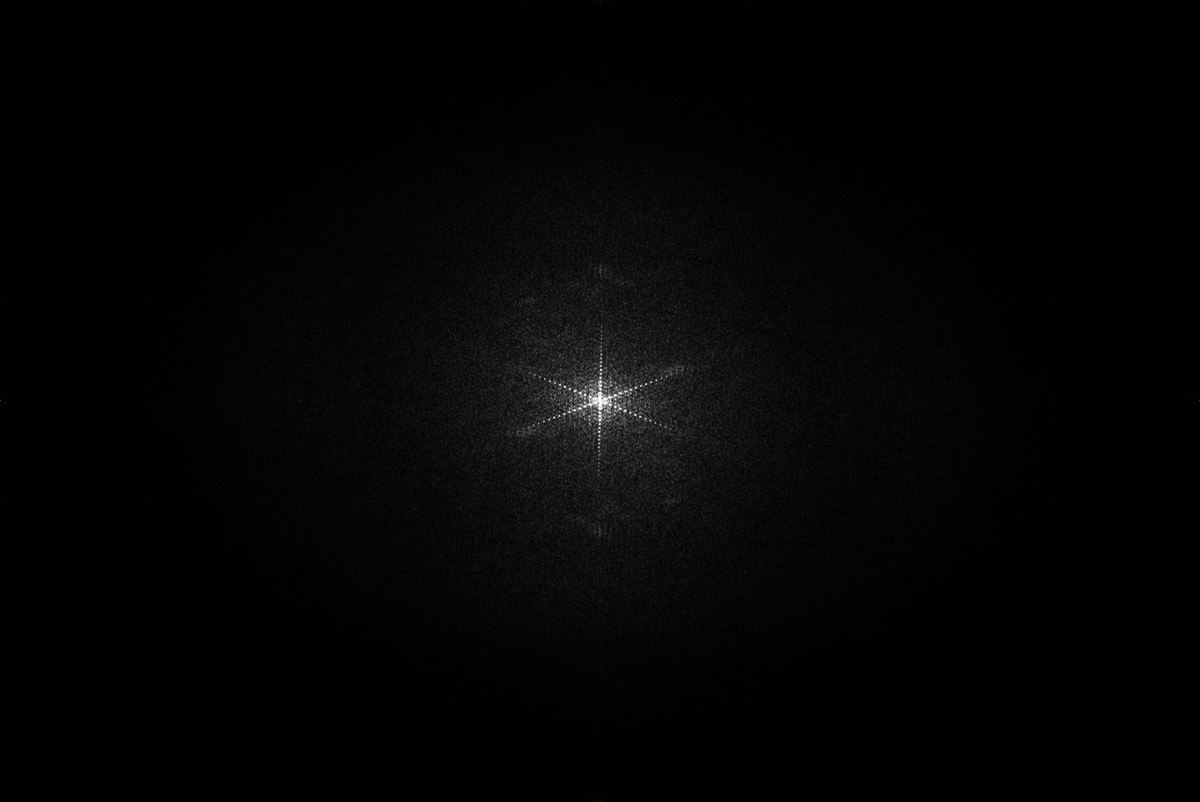
\includegraphics[ width = 0.95 \linewidth ]{figures/CalculatedFT/1549_FT_LinearPlot.png}
        \caption{The calculated FT with no aperture involved}
    \end{minipage}%
    \hspace{0.5cm}
    \begin{minipage}[t]{0.45\textwidth}
        \centering
        
\includegraphics[ width = 0.95 \linewidth ]{figures/CalculatedFT/1548_FT_LinearPlot.png}
        \caption{The calculated FT using the aperture with a diameter of $2.0 \ \si{mm}$}
    \end{minipage}%
    \vspace{1.5cm}
    \begin{minipage}[t]{0.45\textwidth}
        \centering
        
\includegraphics[ width = 0.95 \linewidth ]{figures/CalculatedFT/1547_FT_LinearPlot.png}
        \caption{The calculated FT using the aperture with a diameter of $1.0 \ \si{mm}$}
    \end{minipage}%
    \hspace{0.5cm}
    \begin{minipage}[t]{0.45\textwidth}
        \centering
        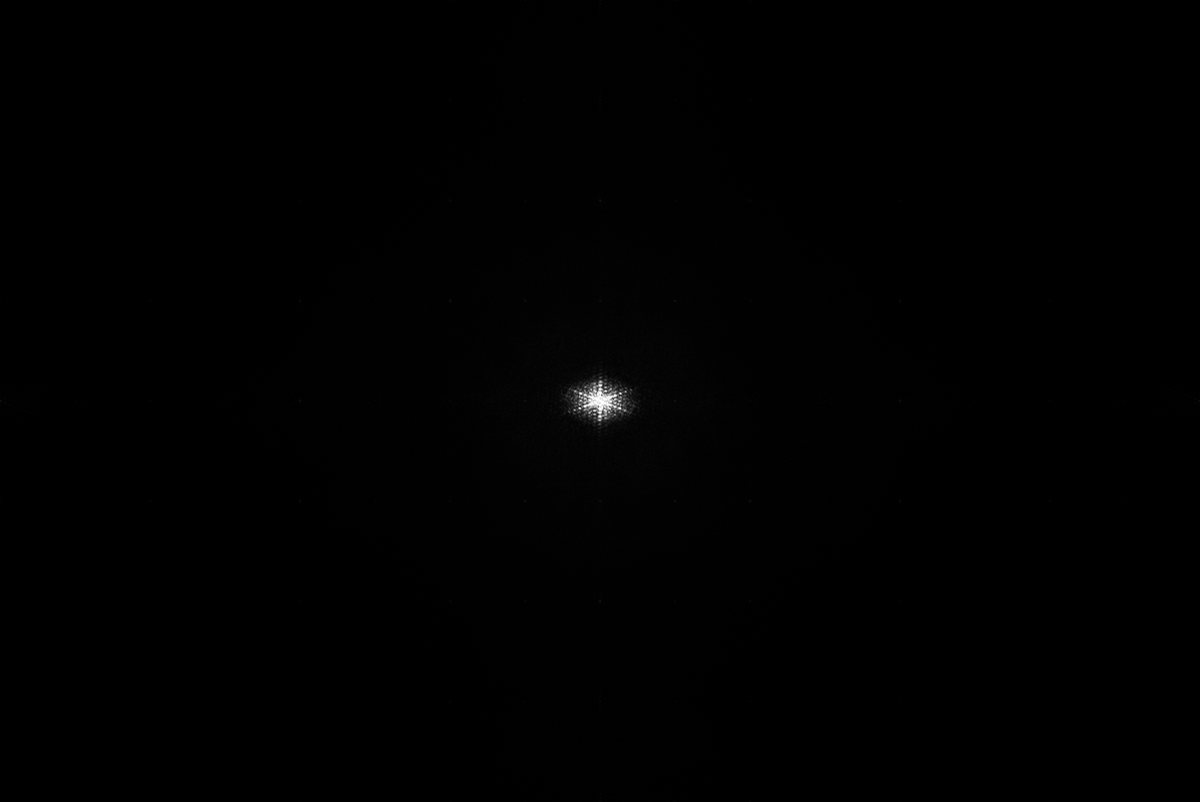
\includegraphics[ width = 0.95 \linewidth ]{figures/CalculatedFT/1546_FT_LinearPlot.png}
        \caption{The calculated FT using the aperture with a diameter of $0.70 \ \si{mm}$}
    \end{minipage}%
    \vspace{1.5cm}
    \begin{minipage}[t]{0.45\textwidth}
        \centering
        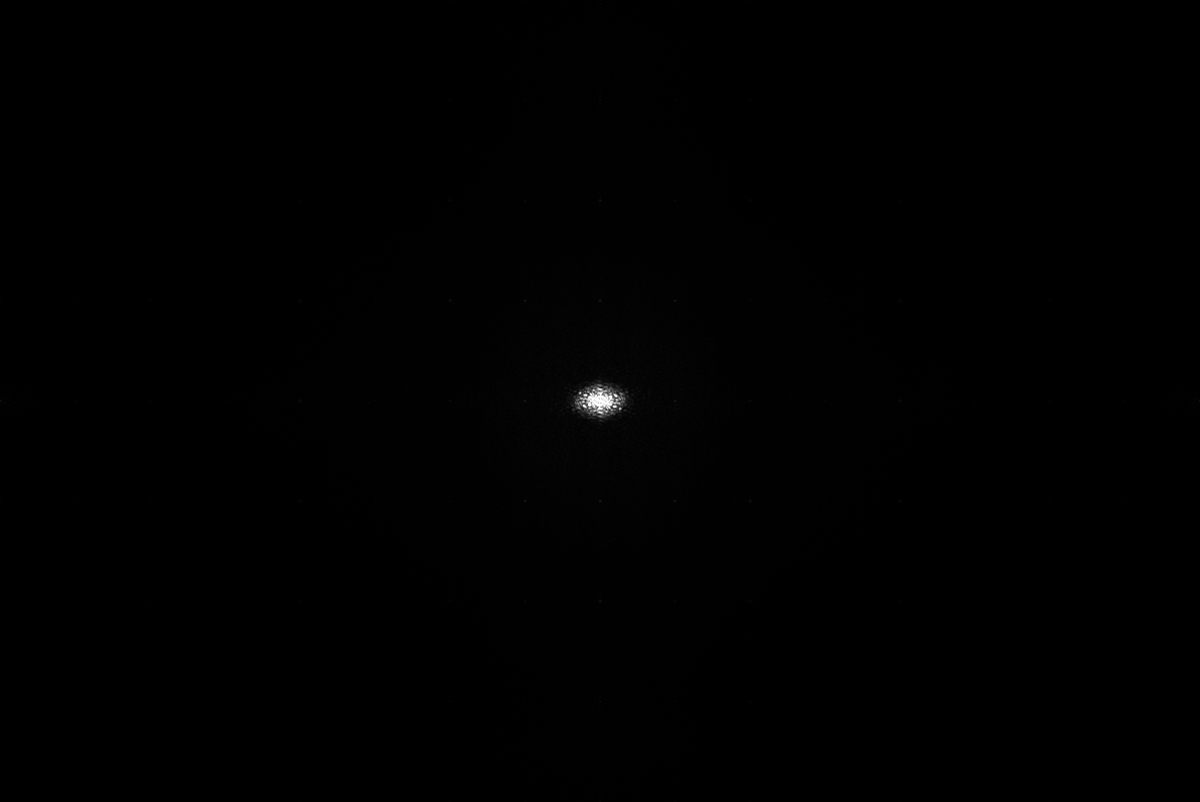
\includegraphics[ width = 0.95 \linewidth ]{figures/CalculatedFT/1545_FT_LinearPlot.png}
        \caption{The calculated FT using the aperture with a diameter of $0.50 \ \si{mm}$}
    \end{minipage}%
    \hspace{0.5cm}
    \begin{minipage}[t]{0.45\textwidth}
        \centering
        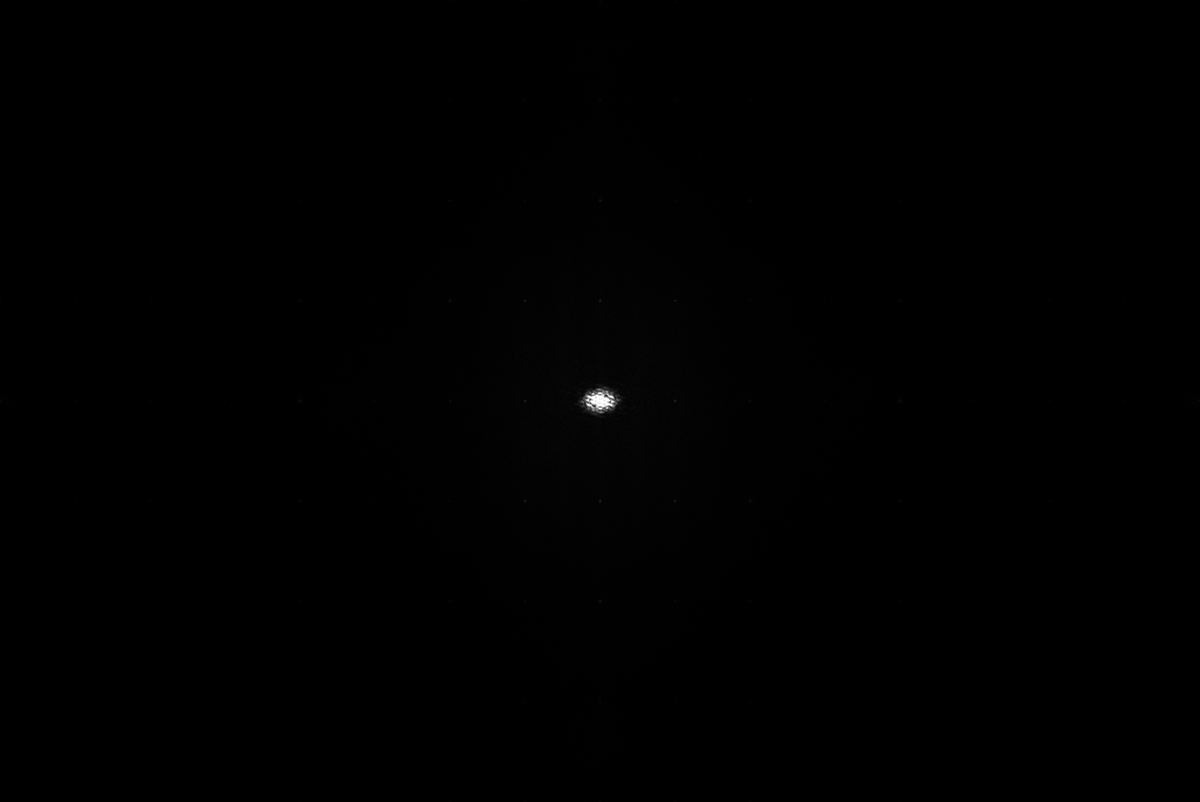
\includegraphics[ width = 0.95 \linewidth ]{figures/CalculatedFT/1544_FT_LinearPlot.png}
        \caption{The calculated FT using the aperture with a diameter of $0.30 \ \si{mm}$}
    \end{minipage}%
\end{figure}